% 
% Compile with ./build.sh
% 

\documentclass{beamer}

\usetheme{Madrid} 

%\usetheme{JuanLesPins}

\usepackage{listings}                                   
\usepackage{hyperref}
\usepackage{graphicx}                                 
\usepackage{tabularx}
\usepackage{microtype}
\usepackage[T1]{fontenc}
\usepackage[scaled]{beramono}
\usepackage{minted}
\usepackage{xcolor}
\usepackage{pgfplots}
\usepackage{dirtytalk}
\usepackage{tikz}
\usetikzlibrary{tikzmark,fit}

%\usepackage{enumitem}
\pgfplotsset{compat=1.6} 

\newcommand\Small{\fontsize{5}{5.2}\selectfont}
\newcommand*\LSTfont{\Small\ttfamily\SetTracking{encoding=*}{-60}\lsstyle}
\renewcommand{\footnotesize}{\tiny}

\hypersetup{colorlinks=color, linkcolor=black}
\definecolor{OliveGreen}{rgb}{0,0.6,0}
\graphicspath{{./images/}}
% 
% Turn off beamer nav stuff...
% 
\setbeamertemplate{navigation symbols}{}


%\input{lst-config/clojure-config}
\begin{document}

\begin{frame}
  \frametitle{Invest In Learning Immutable Tech}
  \center{
    %
    % Graphic for Title Page
    %
    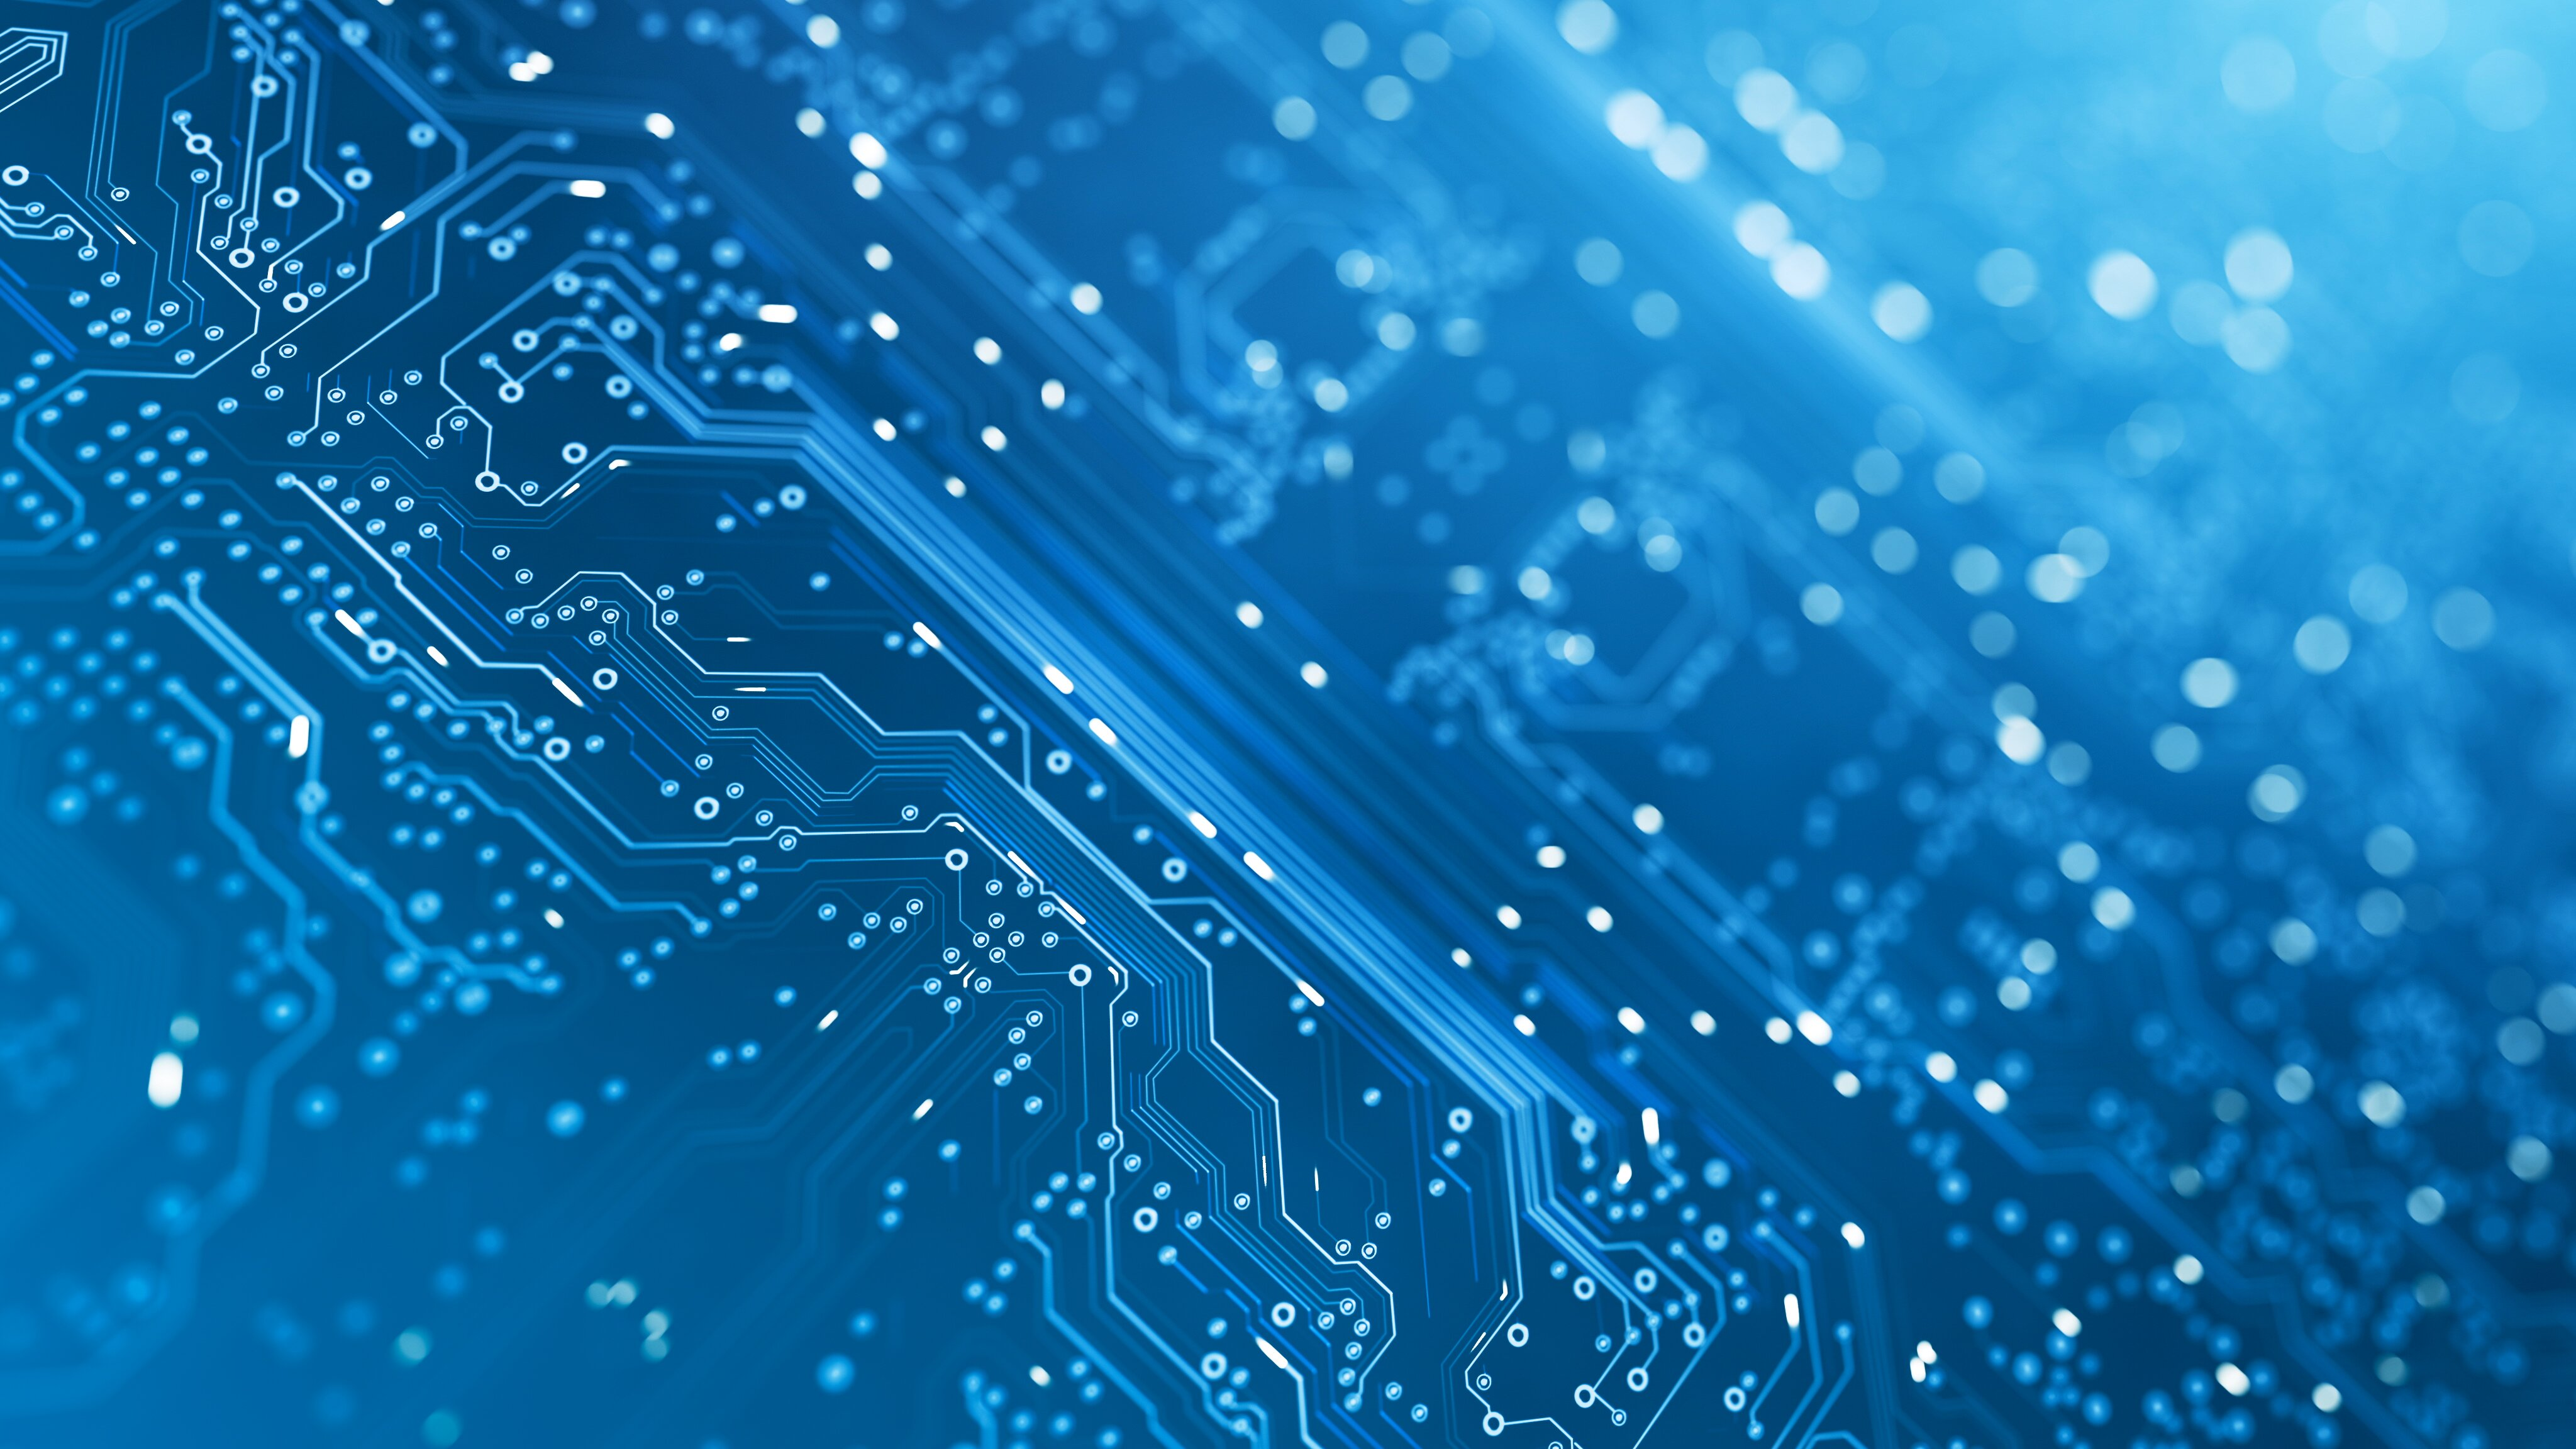
\includegraphics[scale=.15]{tech2}
    
  }
\end{frame}

\frame{
  \frametitle{Change is Inevitable}
  \huge
  \say{To improve is to change; to be perfect is to change often.}
  \large
  \rightline{{\rm  --- Winston Churchill}}
}

\frame{
  \frametitle{Change is Inevitable?}
  \huge
  \say{The more things change, the more they stay the same.}
  \large
  \rightline{{\rm  --- Jean-Baptiste Alphonse Karr}}
}

\frame{
  \frametitle{Once Popular Tech}
   \begin{columns}
    \begin{column}{.49\textwidth}
      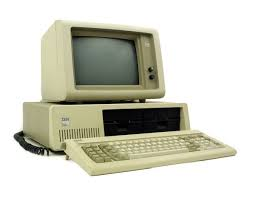
\includegraphics[scale=.50]{ibm-pc}
    \end{column}
    \begin{column}{.49\textwidth}
      \itemize{
      \item CORBA	
      \item COM
      \item DCOM
      \item Adobe Flash
      \item J2EE (Websphere/Weblogic)
      \item Backbone
      \item Ember
      \item Knockout
      \item JQuery
      \item SOAP
      }
    \end{column}
  \end{columns}
}

%\resetcounter[footnote]
%\setcounter{footnote}{0} 


%
% For databases, mention stack-overflow and wikipedia as examples where 
% relational can be web scale
%
\frame{
  \frametitle{Database}
  \begin{columns}
    \begin{column}{.49\textwidth}
      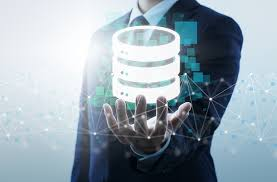
\includegraphics[scale=.615]{db}
      \vfill
      
\includegraphics[scale=.62]{sql}  
    \end{column}
    \begin{column}{.49\textwidth}
      \itemize{
      \item Postgres
      \item SQL Server
      \item Oracle
      \item SQLite
      \item Couchbase
      \item Cassandra
      \item DynamoDB
      \item Bigtable
      \item Snowflake
      \item DB2
      \item H2
      \item MySQL
      %  \footnote{\href{https://www.ics.uci.edu/~lopes/teaching/inf212W12/readings/church.pdf}
      %    {An Unsolvable Problem of Elementary Number Theory}}
      }

    \end{column}
  \end{columns}
  % \center{
  %   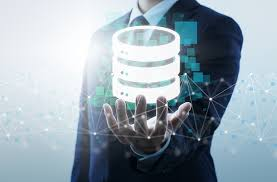
\includegraphics[scale=.75]{db}
    
  }

\frame{
  \frametitle{Operating Systems}
  \begin{columns}
    \begin{column}{.49\textwidth}
      
\includegraphics[scale=.13]{operating-systems}
    \end{column}
    \begin{column}{.49\textwidth}
      \itemize{
      \item Trouble Shooting
      \item Debugging
      \item Performance Tuning
      \item Productivity
      %  \footnote{\href{https://www.ics.uci.edu/~lopes/teaching/inf212W12/readings/church.pdf}
      %    {An Unsolvable Problem of Elementary Number Theory}}
      }

    \end{column}
  \end{columns}
  % \center{
  %   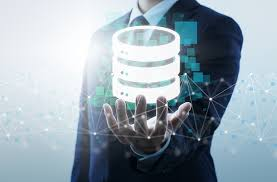
\includegraphics[scale=.75]{db}
    
  }

  \frame{
  \frametitle{Operating System Foundations}
  \begin{columns}
    \begin{column}{.49\textwidth}
      
\includegraphics[scale=.13]{operating-systems}
    \end{column}
    \begin{column}{.49\textwidth}
      \itemize{
      \item Shared Memory
      \item Semaphores
      \item Processes
      \item Threads
      \item Device Drivers
      \item Kernel vs User Space
      \item Sockets
      \item Pipes
      \item File Systems
      %  \footnote{\href{https://www.ics.uci.edu/~lopes/teaching/inf212W12/readings/church.pdf}
      %    {An Unsolvable Problem of Elementary Number Theory}}
      }

    \end{column}
  \end{columns}
  % \center{
  %   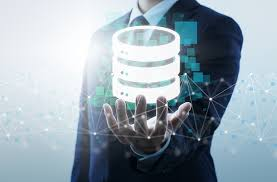
\includegraphics[scale=.75]{db}
    
  }

% \frame{
%   \frametitle{Title - Page of Items}
%   \begin{itemize}
%   \item Item 1
%   % To not show following item until keypress
%   % \pause
%   \item Item 2
%   \item Item 3
%   \end{itemize}
% }




  \frame{
    \frametitle{Networking}
    \begin{columns}
      \begin{column}{.49\textwidth}
        
\includegraphics[width=0.90\textwidth]{networking}
      \end{column}
      \begin{column}{.49\textwidth}
        \itemize{
        \item TCP Transmission Control Protocol
        \item UDP User Datagram Protocol
        \item HTTP Hypertext Transfer Protocol
        \item SFTP Secure File Transfer Protocol
        \item SSL Secure Socket Layer
        \item DHCP Dynamic Host Configuration Protocol 
        \item DNS Domain Name System
        % {\href{https://www.rfc-editor.org/rfc-index.html}
        % {RFC Index}}
        }
      \end{column}
    \end{columns}
    % \center{
    %   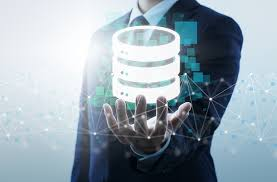
\includegraphics[scale=.75]{db}
      
    }

    %% TODO - add JVM and ASM Slides


%https://clojure.org/api/cheatsheet
\frame{
  \frametitle{Resources}
  \begin{itemize}

  \item \href {https://www.rfc-editor.org/rfc-index.html}{\color {blue}{RFC Index}}
  \item \href {https://developer.arm.com/documentation/107829/0200/Assembly-language-basics}{\color {blue}{ARM Assembly Language}}
  \item \href {https://www.youtube.com/watch?v=OT1RErkfLNQ}{\color {blue}{SQL - Beginner to Advanced in 4 hours}}
  \item \href {https://www.clojure.org}{\color {blue}{Clojure}}
  \item \href {https://github.com/tstout/presentations/blob/main/immutable-tech/immutable-tech.tex}{\color {blue}{Source Code For This Document}}

    %% put a ref to this https://github.com/chubin/cheat.sh
  \end{itemize}
}

\end{document}
